%%% Local Variables:
%%% mode: latex
%%% TeX-master: "report"
%%% End:

Many motion planning algorithms exploit topology in the free space to help design efficient motion planners or produce concise maps. Most of those works have utilized the generalized Voronoi diagram (GVD), which is a topological map that can be embedded into the free space.
A \emph{topological map} usually is used to describe a graph in where the nodes correspond to distinct position and edges represent paths between different positions in robotics. In 2003, Choset and Rizzi explored that a topological map is not only a graph but carries more information and may actually be used to perform task decompositions~\cite{DBLP:conf/isrr/ChosetR03}.

\subsection{Good Topological Maps}
The topological map \(M\) for a free space \(X\) is a map that every homotopy class of \(X\) has a corresponding homotopy class in \(M\). Moreover, if the fundamental group of \(M\) is isomorphic to the fundamental group of the free space, we say \(M\) is a \emph{good topological map}. For example, for \(2\)-dimensional problems the generalized Voronoi diagram is a good map. See Figure~\ref{fig:gvd}. Analogously, a topological map contains redundant loops which do not have corresponding loops in the free space is \emph{bad}.
\begin{figure}
  \centering
  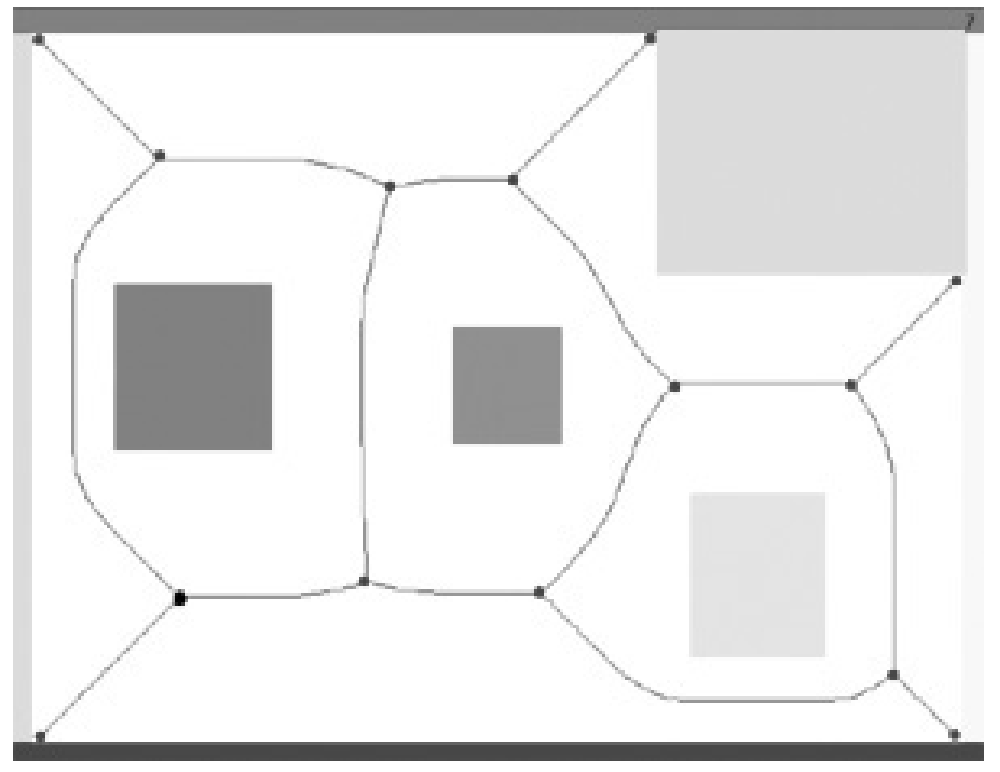
\includegraphics[width=0.5\textwidth]{fig-gvd}
  \caption{An example of good topological map, the rectangles represent the obstacles}
  \label{fig:gvd}
\end{figure}

Some topological map is the abstraction of a \(1\)-dimensional roadmap, which is geometric structures embedded in the free space with three properties: accessibility (it is possible to plan a path between two points onto the roadmap), connectivity (move towards the vicinity of the target point along the roadmap), and departability (reach the target).
To see why the roadmap needs to be only \(1\)-dimensional, consider a point-GVD \(G\) in \(\R^3\), \(G\) consists of \(2\)-dimensional manifolds. The overlap of these \(2\)-dimensional sheets is a \(1\)-dimensional structure called the generalized Voronoi graph (GVG) that the distance from any point in it to adjacent three obstacles are same~\cite{choset1996sensor}. Although the GVG satisfies accessibility and departability, it is not guaranteed to be connected in general. In 1995, Choset and Burdick introduced an extension of GVG called the hierarchical generalized Voronoi graph (HGVG), which is also retract-like. But the later is connected under certain conditions in~\cite{choset1996sensor}. Therefore, it could be used to produce the roadmap for performing a motion planning algorithm. For the detail of how to construct such a HGVG incrementally, see~\cite{choset1995sensor}.

However, generally speaking, the roadmaps mentioned above hardly be good topological maps, and there is no \(1\)-dimensional retract for space of dimensions greater than \(2\). In other words, it is hard to generate good topological maps for \(\R^m\) with \(m>2\).

\subsection{Task Decomposition}
According to the definition of good topological map above, restracts work as good maps because the retraction naturally offers the accessibility, departability, and the retract is connected in every connected components of the free space by the continuity of the retraction function. Moreover, it preserves the cardinality of the first fundamental group as well.

As pointed earlier, we cannot define a \(1\)-dimensional retract of a space with dimension at least \(3\). Nevertheless, a topological map of a \(2\)-dimensional work space can be used to decompose a multi-dimensional configuration space into a set of contractible regions.
Therefore, we can find good maps through retraction in each region and put them back together through the topological adjacency relationship from the original work space. The result is called \emph{piecewise retract} by Choset and Rizzi. Notice that although the piecewise retract may be a bad topological map most times, it consists of smaller good maps for subsets of the configuration space and thus works well for a motion planner.
For examples of applications of piecewise retract, see~\cite{DBLP:conf/isrr/ChosetR03}.